\documentclass[tikz, border=0mm, convert={density=300,size=1080x800, outext=.png}]{standalone}
\usepackage{amsmath}
\usepackage[most]{tcolorbox}
\usetikzlibrary{backgrounds}

\begin{document}
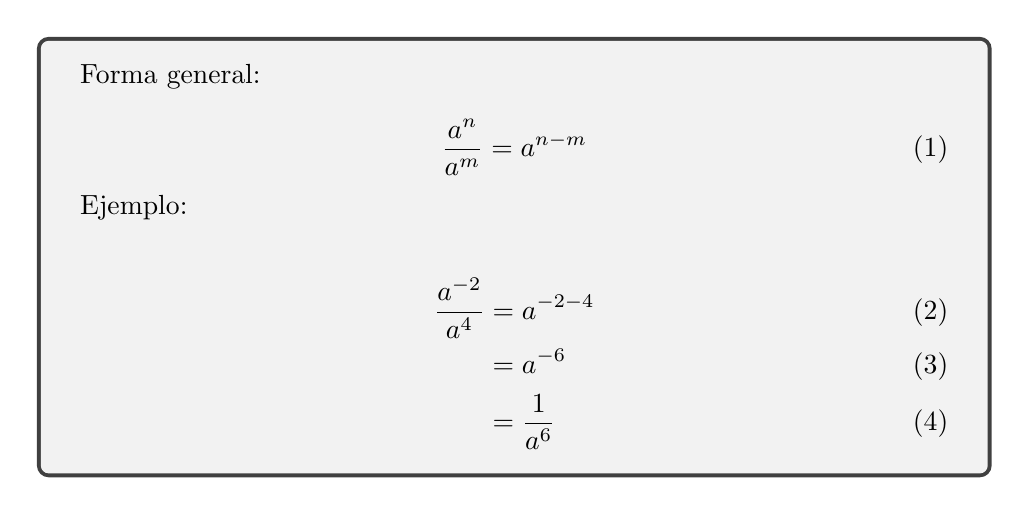
\begin{tikzpicture}[auto]
\node at (0,0) {%
\begin{tcolorbox}
    Forma general:
    
    \begin{equation}
        \frac{a^n}{a^m} = a^{n-m}
    \end{equation}
        
    Ejemplo:
    
    \begin{align}
        \frac{a^{-2}}{a^4} &= a^{-2-4} \\ 
        &= a^{-6} \\ 
        &= \frac{1}{a^6} 
    \end{align}
\end{tcolorbox}
};
\end{tikzpicture}
\end{document}